% --WordPress--
\chapter{Sito in WordPress}
\label{chp:wp}

L'analisi dei requisiti ha evidenziato la necessità di un sito web in cui esporre e descrivere al cliente i servizi offerti, aggiornato e popolato da un componente del team di {\fem} senza per forza conoscenze e capacità tecniche informatiche; si é scelto quindi WordPress, un CMS molto diffuso.

{\wp} è una piattaforma software di content management system (CMS) ovvero un programma installato sul server che consente la creazione, gestione, distribuzione e manutenzione di un sito Internet \cite{wordpress}. É un progetto open-source creato da Matt Mullenweg e distribuito con la licenza GNU General Public License; é sviluppato in PHP con appoggio a MySQL come gestore di database.

{\wp} permette il download gratuito di tutti i suoi componenti dal sito \url{www.wordpress.org} per poterli installare sulla propria macchina. Esiste anche un servizio (a pagamento in base alle richieste) chiamato \emph{WordPress.com} che permette di costruire rapidamente il proprio sito web o blog basato su {\wp} senza la necessità di possedere un server o competenze tecniche specifiche.

\section{Caratteristiche di {\wp}}
{\wp} permette di estendere le proprie funzionalità con l'ausilio di opportuni plugin, ovvero moduli che aggiungono nuove caratteristiche ed elementi all'applicativo. I plugin possono essere gratuiti o a pagamento e possono fare molte fare di tutto, dal potenziare l'editor integrato di {\wp} all'inserire slideshow nelle pagine, e molto altro ancora. Come i plugin si possono trovare anche temi, estensioni che permettono di personalizzare l'aspetto del sito modificando sfondi, impaginazione, font, etc.

\section{{\wp} per avifauna.fem2ambiente.com}
Per realizzare il \emph{Portale della Diagnostica Molecolare dedicato all'Avifauna}, dopo aver scelto il sottodominio \texttt{www.avifauna.fem2ambiente.com}, si é prima di tutto installato e configurato {\wp}.

Per farlo é stato necessario scaricare l'ultima versione dal sito \url{www.wordpress.org} (ad oggi, Ottobre 2015, l'ultima versione é la 4.3.1) e seguire le istruzioni nel file \texttt{readme} \cite{installing_wordpress}, in particolare:
\begin{itemize}
\item eseguire le opportune modifiche al file \texttt{wp-config.php} in un editor di testo;
\item creare un database dedicato utilizzando MySQL;
\item connettersi al server e caricare tutti i file relativi l'installazione di {\wp} nella cartella scelta (\texttt{/home});
\item configurare in modo appropriato visitando la pagina 

\texttt{http://avifauna.fem2mabiente.com/home/wp-admin/install.php}
\end{itemize}

Una volta terminata l'installazione si é potuto procedere con l'installazione degli appropriati plugin, temi e estensioni.

La scelta del tema é ricaduta su \emph{Everest} di YOOtheme (Versione: 1.0.11). YOOtheme é una azienda tedesca che produce componenti per CMS \cite{yootheme}; i loro prodotti più importanti, oltre a una ventina di temi e template diversi rispettivamente per {\wp} e Joomla!, sono \emph{Wrap Framework} \cite{wrap} e \emph{Uikit} \cite{uikit}, due architetture software di supporto per la creazione e personalizzazione dei componenti aggiuntivi ai più famosi CMS.

Il tema Everest é stato costruito utilizzando Wrap Framework e mette a disposizione dell'utilizzatore sette stili di layout differenti, personalizzazioni nella costruzione del layout sfruttando tutte le potenzialità di {\wp} e un pacchetto di plugin chiamato \emph{Widgetkit} per l'inserimento rapido di Slideshow, gallierie di immagini, mappe. Per tutte queste caratteristiche é stato scelto, acquistato ed installato come tema per il sito.

Per ricoprire tutti i bisogni organizzativi di un sito commerciale come il Portale Avifauna é stato necessario installare anche plugin come \emph{Polylang} \cite{polylang} per il supporto multilingue al sito e \emph{My Calendar} \cite{mycalendar} per la gestione degli eventi.

Dopo aver creato popolato il sito con i contenuti, divisi in base alle pagine e sezioni dedicate, il risultato ottenuto é visibile nell'immagine~\ref{fig:homepage} e al seguente link \url{www.avifauna.fem2mabiente.com/home}.

\begin{figure}
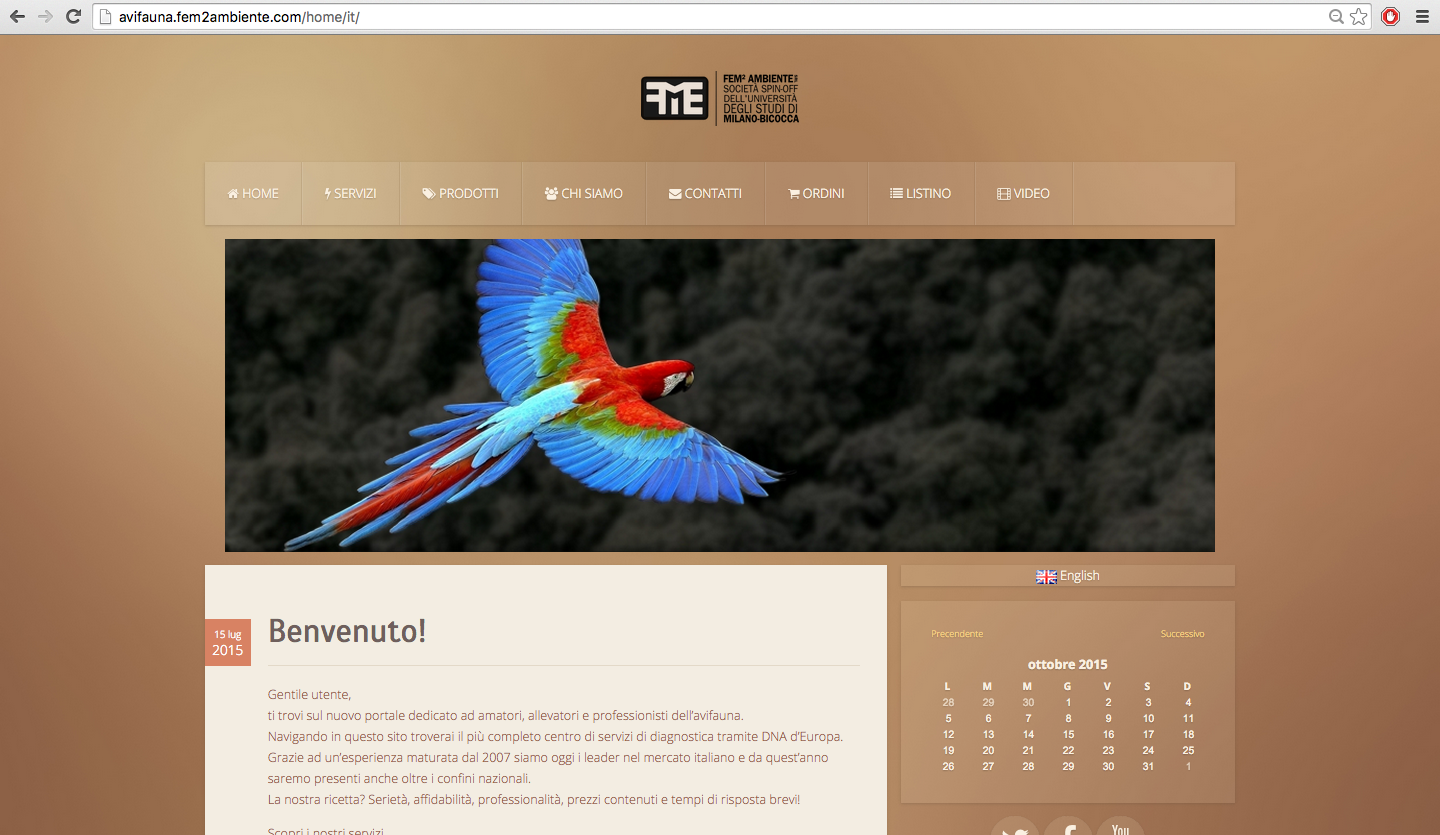
\includegraphics[width=1\textwidth]{images/homepage} 
\caption{homepage del Portale per la Diagnostica Molecolare Avifauna}
\label{fig:homepage}
\end{figure}

Cliccando sul tasto \textsf{Ordini} si può accedere alla piattaforma personalizzata, descritta nei seguenti capitoli.

\begin{center}

\includegraphics[width=0.3\textwidth]{images/homepage-ordini} 
\label{fig:homepage-ordini}
\end{center}

% --Sviluppo Piattaforma--
\chapter{Sviluppo Piattaforma Web}
\label{chp:sviluppo}
In questo capitolo é descritta la costruzione della piattaforma acquisti associata al sito divulgativo creato con {\wp}. Lo sviluppo può essere concettualmente diviso in due parti: il \emph{lato server} e il \emph{lato client}. Esse si concentrano rispettivamente sulla creazione di una base su cui interagire per tenere traccia di tutte le azioni compiute nel flusso di acquisto e analisi e sull'interfaccia con l'utente finale, che può essere il cliente oppure un addetto di {\fem}.

% --Lato Server--
\section{Lato Server}
\label{sec:server}
Per lo sviluppo della piattaforma web le tecnologie utilizzate sono state: \emph{Django} come web framework e \emph{MySQL} per il database.

\subsection{Django}
\label{subs:django}
\emph{Django} è un web framework open source per lo sviluppo di applicazioni web, scritto in linguaggio \emph{Python}; il progetto è sviluppato dalla "Django Software Foundation" (DSF), un'organizzazione indipendente senza scopo di lucro \cite{django}. É stato inizialemente concepito per gestire diversi siti di notizie, ed in seguito distributo con una licenza BSD (Berkeley Software Distribution) a luglio 2005.

La scelta di Django é ricaduta grazie alle molte proprietà: dall'astrazione del database relazionale ad oggetti, alla
possibilità di installare funzionalità attraverso plugin, dalla robusta API per la gestione del database, al sistema di "view generiche" che evitano la stesura di codice ripetitivo per determinati casi comuni e soprattutto il sistema di template  e gestore di URL basate su espressioni regolari. Django offre inoltre un efficace supporto per localizzazione, incluse traduzioni dell'interfaccia amministrativa in molte lingue.

\subsection{Configurazione}
\label{subs:config}
Il primo passo é stato l'installazione delle componenti di Django, attraverso la creazione del progetto (nome di esempio \texttt{mysite}), con il comando a terminale:
\begin{verbatim}
$ django-admin startproject mysite
\end{verbatim}

così da ottenere la seguente configurazione di file:
\begin{small}
\begin{verbatim}
mysite/
    manage.py
    mysite/
        __init__.py
        settings.py
        urls.py
        wsgi.py
\end{verbatim}
\end{small}

Abbiamo quindi impostato nel file \texttt{settings.py} il database scelto, le lingue del sistema, il percorso dei file statici, dei media e le \texttt{INSTALLED\_APPS}.

Le \texttt{INSTALLED\_APPS} sono una sorta di librerie usate per l'aggiunta di componenti al progetto costruito; le più importanti sono:
\begin{itemize}
 \item \texttt{django.contrib.admin} - il creatore automatico del pannello admin
 \item \texttt{django.contrib.auth} - il sistema di autenticazione
 \item \texttt{django.contrib.sessions} - il framework per il controllo delle sessioni
 \item \texttt{django.contrib.messages} - il framework di controllo per i messaggi
 \item \texttt{django.contrib.staticfiles} - il gestore dei "file statici"
\end{itemize}

\subsection{Creazione}
\label{subs:crea}
Durante tutta la fase di sviluppo é stato necessario avviare il \emph{development server} attraverso il comando da terminale:
\begin{verbatim}
$ python manage.py runserver
\end{verbatim}
per simulare il comportamento del server in modo da generare il sito all'indirizzo \texttt{http://127.0.0.1:8000/} .

Una componente fondamentale é rappresentata dai \emph{modelli}, strutture associabili concettualmente alle classi in Java; in funzione alle richieste avanzate da {\fem} il diagramma in figura~\ref{fig:modelli} rappresenta come sono stati configurati i modelli con i relativi attributi.

\begin{figure}
 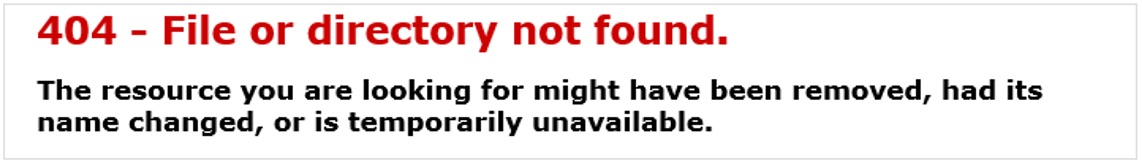
\includegraphics[width=1\textwidth]{images/filenotfound} 
 \caption{configurazione modelli}
 \label{fig:modelli}
\end{figure}

nei seguenti paragrafi sono descritti i principali modelli.

\subsection*{clienti.py}
\label{subs:clienti}
Il cliente é un componente delicato ed importante del sistema. 

L'attributo \texttt{tipo} é necessario in quanto per {\fem} il cliente può essere differenziato in quattro tipi: Amatore, Allevatore, Veterinario e Negozio. Esso é identificato univocamente dall'indirizzo \texttt{email} inserito al momento della registrazione e ha chiaramente un attributo \texttt{ragione\_sociale} per indicare nome e cognome per un privato, oppure ragione sociale in caso contrario. Ogni cliente ha altri numerosi attributi per ogni dato personale relativo all'indirizzo (necessario per la spedizione degli attestati generati al termine delle analisi), contatti telefonici e \texttt{lingua\_preferita} per tradurre il sistema correttamente.

Ogni cliente può acquistare pacchetti di \emph{Crediti FEM}, cioè una somma di denaro pronta per gli acquisti pagata anticipatamente, in modo da non dover effettuare il pagamento al termine di ogni ordine, é quindi necessario indicare la quantità di crediti posseduta da ogni cliente in un apposito attributo.

Infine ogni cliente può essere iscritto ad una associazione convenzionata all'azienda {\fem} e deve poter inserire il proprio numero di tessera per accedere agli sconti relativi; per farlo si deve dare uno sguardo ai modelli \texttt{associazioni.py} e \texttt{prezzi.py}.

\subsection*{prezzi.py}
\label{subs:prezzi}
Ogni \texttt{SchemaPrezzi} é identificato dal \texttt{nome} e può essere associato a nessuno, uno o tanti clienti. Esso definisce i costi fissi delle commissioni per ogni metodo di pagamento scelto, il prezzo degli attestati e il prezzo di ogni analisi, che tendenzialmente può variare tra uno SchemaPrezzi e l'altro.
In particolare abbiamo deciso di differenziare gli SchemaPrezzi secondo una caratteristica principale: se schema \emph{Pacchetti} o \emph{Convenzioni}.

Uno SchemaPrezzi del tipo \emph{Pacchetti} é caratteristico di un cliente standard, che può usufruire di sconti vincolati a quantità, ad esempio con l'acquisto di un analisi APV associato ad un analisi SMAP riduce il costo di entrambe. Uno SchemaPrezzi del tipo \emph{Convenzioni} invece é adatto per i clienti che risultano iscritti ad una associazione che ha attiva una convenzione con {\fem}; questo tipo di SchemaPrezzi modifica il prezzo di tutte o alcune analisi anche in relazione alle specie del campione scelta.

\subsection*{associazioni.py}
\label{subs:associazioni}
Una \texttt{Associazione} é caratterizzata da un nome e da uno schema prezzi associato. \texttt{IscrizioneAssociazione} indica la correlazione tra un cliente, indicato attraverso nome e numero di tessera, e una associazione.

\subsection*{ordini.py}
\label{subs:ordini}
L' \texttt{Ordine} é il componente più delicato e complesso del sistema a causa del suo flusso rappresentato in figura~\ref{fig:flusso-ordine}.

\begin{figure}
 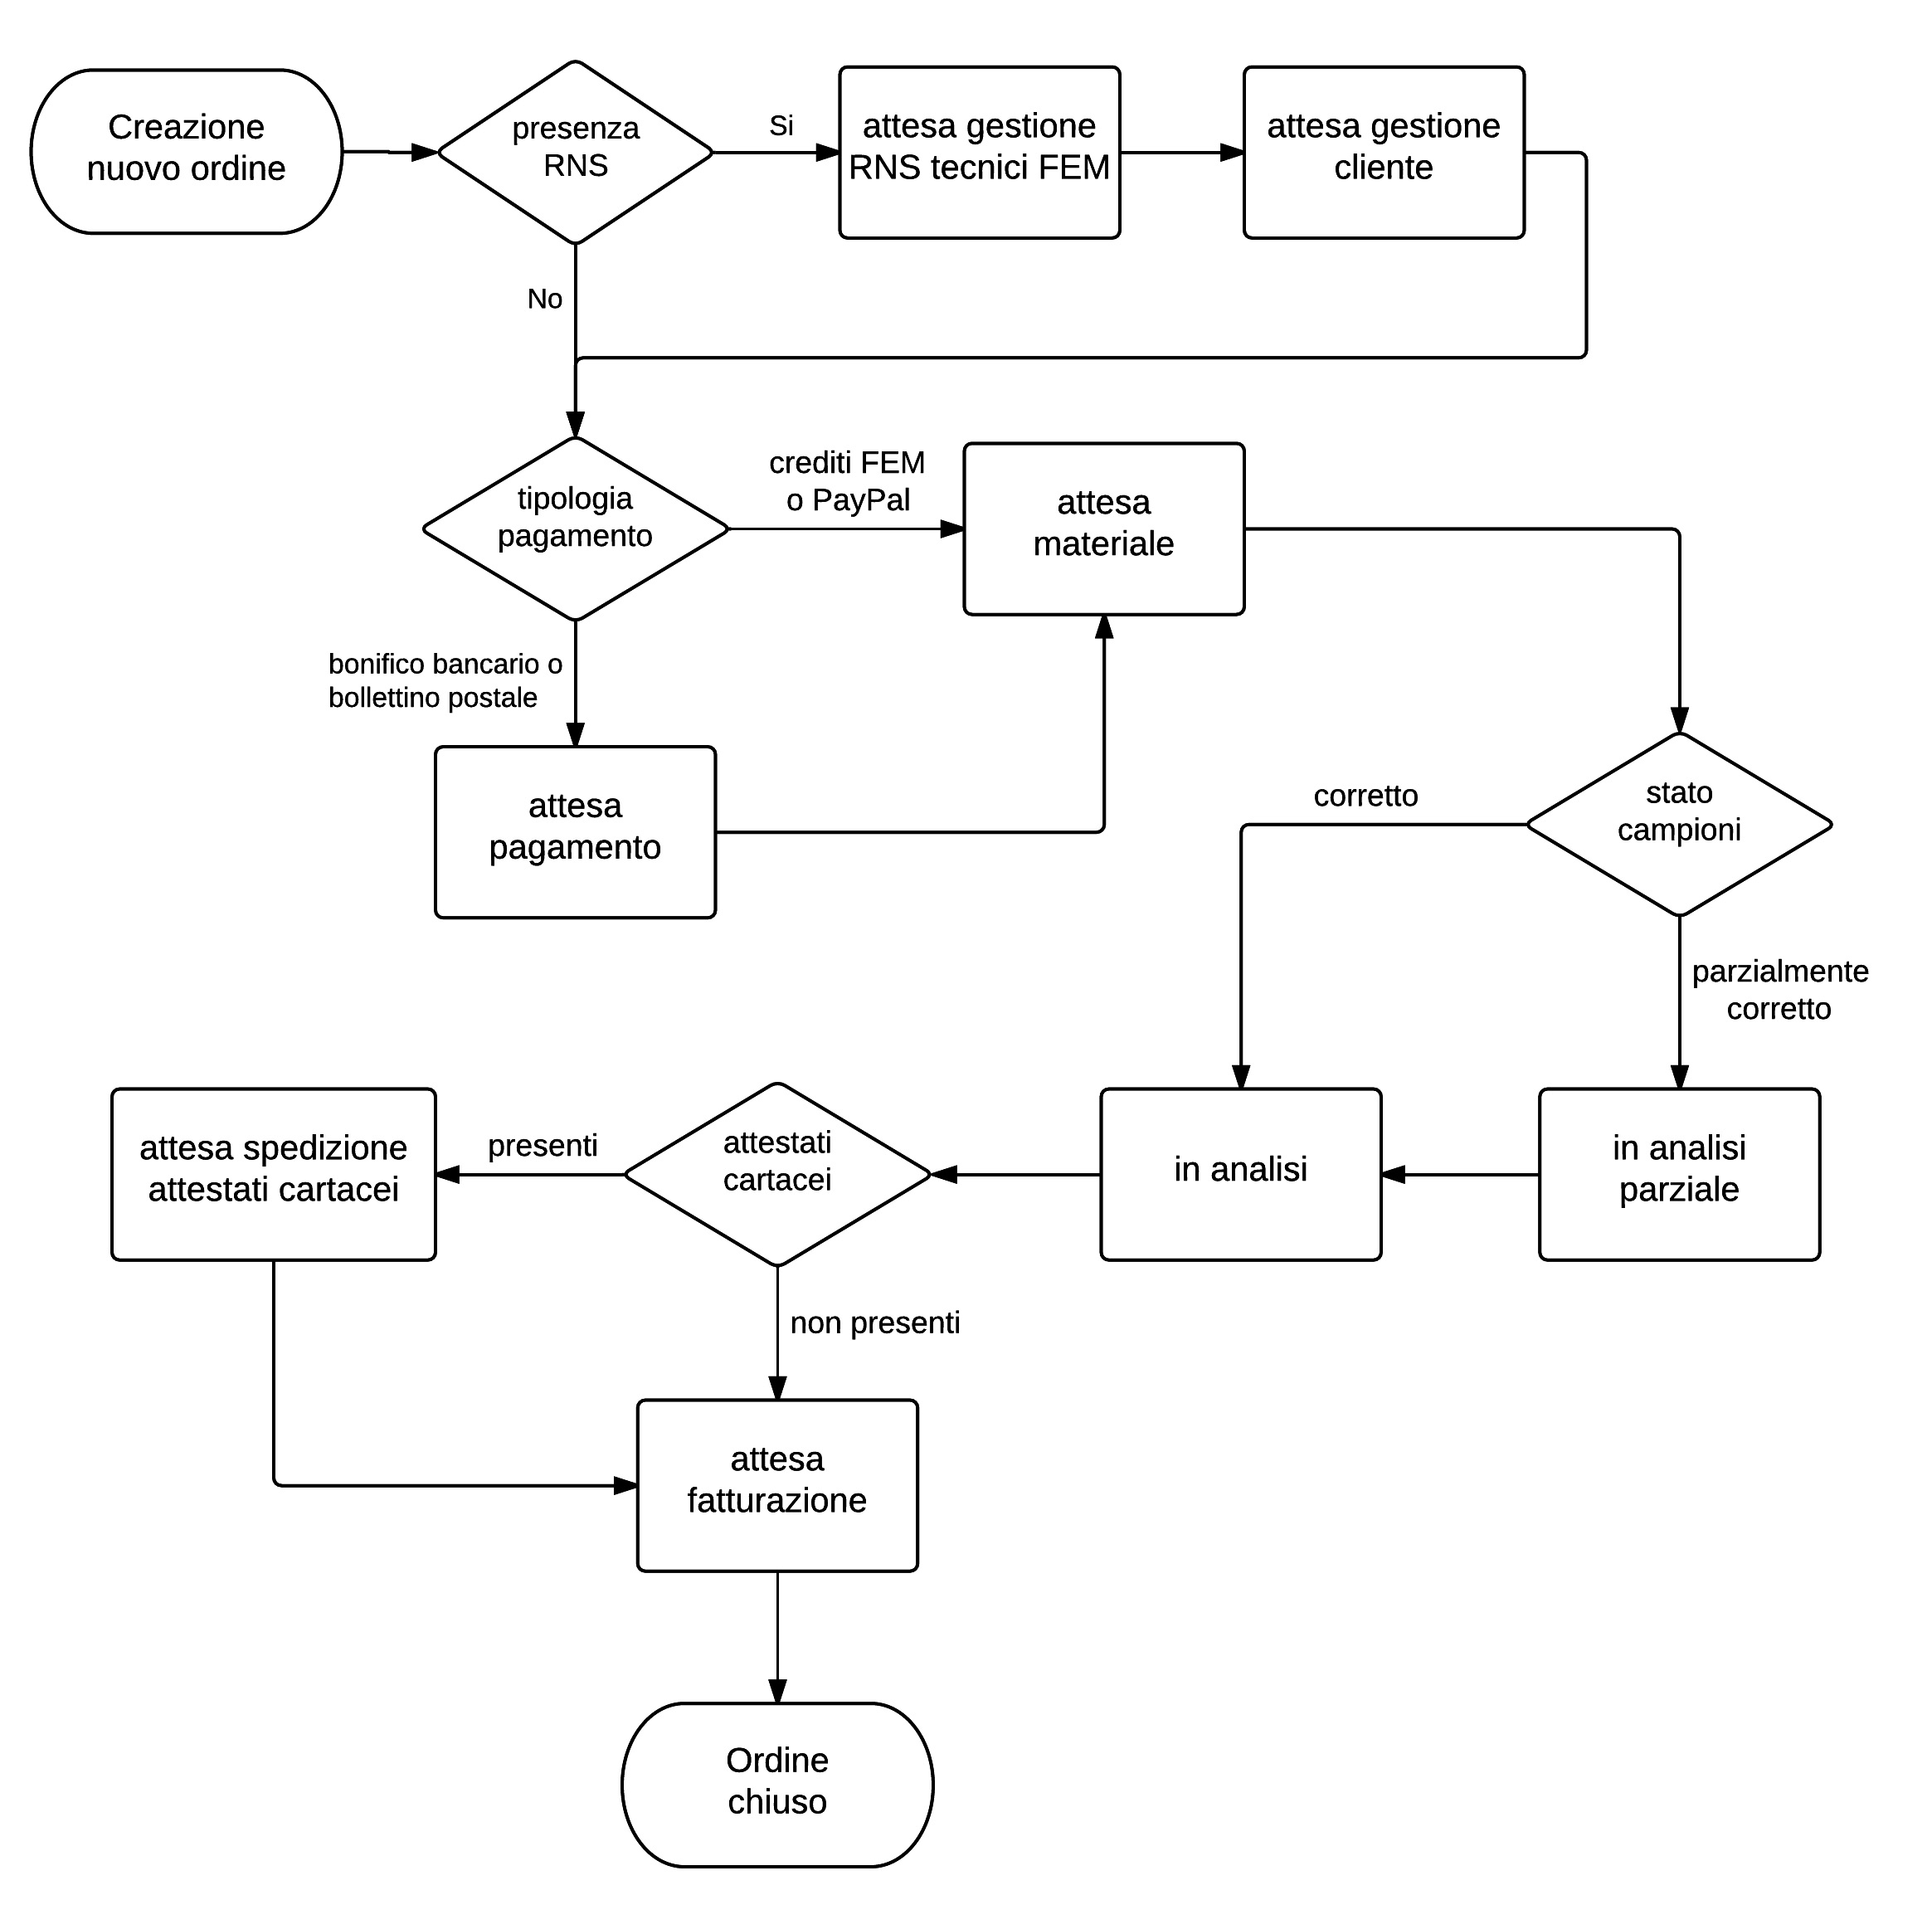
\includegraphics[width=1\textwidth]{images/flusso-ordine} 
 \caption{flusso ordine}
 \label{fig:flusso-ordine}
\end{figure}

Esso é caratterizzato da un numero, dal \texttt{cliente} che l'ha creato e dall''attributo \texttt{stato} che indica in quale posizione del flusso si trova.
Altri attributi interessanti sono:
\begin{itemize}
 \item \texttt{metodo\_pagamento} indica il metodo di pagamento scelto
 \item \texttt{totale\_servizi} indica il costo delle analisi richieste con aggiunte le eventuali spese di spedizione per gli attestati cartacei 
 \item \texttt{crediti\_consumati} indica la quantità di crediti FEM utilizzati per pagare l'ordine
 \item \texttt{servizi\_da\_pagare} indica il  \texttt{totale\_servizi} da cui sono stati sottratti i \texttt{crediti\_consumati}
 \item \texttt{ammontare} indica il \texttt{totale\_servizi} sommato all'eventuale costo di commissione previsto dal metodo di pagamento
\end{itemize}

\subsection*{specie.py}
\label{subs:specie}

É necessario prima di tutto spiegare che la tassonomia (dal greco \emph{taxis} "ordinamento", e \emph{nomos} "norma" o "regola") é definita in generale come la disciplina della classificazione. Abitualmente si impiega il termine per indicare la tassonomia biologica, ossia la disciplina scientifica che si occupa di attribuire un nome agli organismi viventi e di classificarli. La gerarchia di classificazione biologica secondo gli otto principali ranghi tassonomici é descritta in figura~\ref{fig:tassonomia} (le posizioni intermedie alla classifica non sono visualizzate).

\begin{figure}
 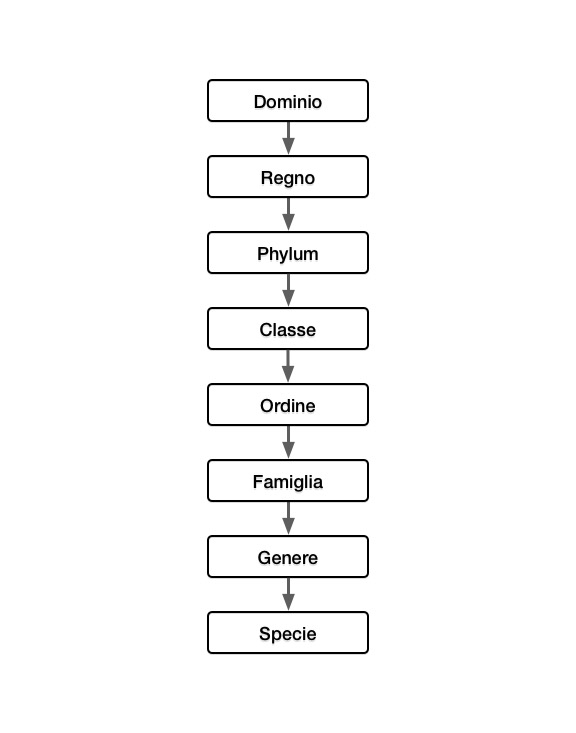
\includegraphics[width=1\textwidth]{images/tassonomia} 
 \caption{Classificazione biologica secondo i principali ranghi tassonomici}
 \label{fig:tassonomia}
\end{figure}

Il Portale Avifauna si occupa per definizione di analisi su un complesso di uccelli che vivono in una determinata regione, ma non tutti gli esemplari richiedono lo stesso tipo di approccio o tecnica per effettuare la analisi. La differenziazione principale scelta é quindi in base a \emph{specie} e sottospecie.

Il modello \texttt{specie.py} si occupa di creare la base per questa differenziazione. Ogni specie ha \texttt{ordine}, \texttt{famiglia} e \texttt{nome} oltre ad un \texttt{immagine} per descriverla; ogni \texttt{sottospecie} ha la \texttt{specie} di riferimento, il \texttt{nome} e i possibili \texttt{nomi\_comuni} e \texttt{protonimi}. 

Le sottospecie sono anche caratterizzate dalla proprietà \texttt{junior} ovvero considerate 'nuove' per {\fem} che non ha ancora acquisito un numero soddisfacente di dati relativi alla sottospecie in questione, quindi non garantisce al 100\% il corretto risultato delle analisi di tipo sessaggio. 

Per facilitare il lavoro in laboratorio sono stati creati anche \texttt{metodo\_di\_estrazione}, \texttt{metodo\_di\_amplificazione}, \texttt{metodo\_di\_visualizzazione} utili ai tecnici per riconoscere più rapidamente come eseguire le operazioni di analisi.

\subsection*{campioni.py}
\label{subs:campioni}
Analogamente ad un e-commerce tradizionale ogni ordine é una sorta di carrello che contiene uno o più oggetti all'interno; nel Portale Avifauna gli oggetti sono i \texttt{campioni}, ovvero gli esemplari su cui sono richieste le analisi da effettuare.

Ogni campione ha i seguenti attributi:
\begin{itemize}
 \item \texttt{ordine} per indicare il numero di ordine di riferimento
 \item \texttt{identificativo} ovvero il nome dell'esemplare
 \item \texttt{specie} o un eventuale \texttt{altra\_specie} in caso in cui non sia presente nell'elenco fornito da {\fem}
 \item \texttt{mutazione}, \texttt{proprietario} e \texttt{data\_di\_nascita} utili soprattutto per la generazione degli attestati
 \item \texttt{lab}, \texttt{problema\_campione}, \texttt{standard}, \texttt{voucher} utili per il lavoro in laboratorio
\end{itemize} 

Il campo \texttt{identificativo} segue le regole fornite dalla \emph{Federazione Ornicoltori Italiani} (F.O.I.), un ente che raggruppa tutti gli appassionati ornicoltori e gli allevatori di uccelli con lo scopo di promuovere lo studio, il miglioramento, lo sviluppo e la conservazione del patrimonio ornitologico \cite{foi}. La F.O.I. ha regolamentato che per poter partecipare alle Manifestazioni Ornitologiche occorre che gli uccelli abbiano alla propria zampa un anellino che riporta i dati dell'allevatore (mediante la sigla \emph{R.N.A.}), l'anno di nascita del soggetto e un numero progressivo, attraverso il quale è possibile risalire ai genitori, contattando l'allevatore che avrà avuto cura di registrare i dati genealogici in appositi registri. Il campo identificativo indicherà quindi il nome dell'esemplare in caso di privati e RNA+Anello in caso di allevatori professionisti.

Per facilitare il lavoro in laboratorio sono stati introdotti gli attributi \texttt{lab} che indica il numero progressivo e univoco in laboratorio e \texttt{problema\_campione} per indicare eventuali caratteristiche del campione, che può essere normale, mancante, inadatto, rischioso o annullato. Altri attributi interessanti sono \texttt{voucher} che funge da 'etichetta' per evidenziare un campione che viene preso di riferimento per future analisi e soprattutto \texttt{standard}.

Una specie, come spiegato precedentemente in~\ref{subs:specie}, può essere definita \emph{junior} in caso in cui {\fem} lo reputi necessario in quanto non ha ancora eseguito un numero minimo di analisi di tipo sessaggio sulla specie in questione per sentirsi fiduciosa da assicurare il successo delle analisi al 100\%. Per questo motivo, al momento della creazione dell'ordine, se viene aggiunto un campione di specie junior, si chiede di aggiungere eventuali campioni (se il cliente ne é in possesso) definiti \emph{standard}, ovvero esemplari di cui il cliente é già a conoscenza del sesso (tipicamente i genitori) in modo da aumentare le possibilità di successo delle analisi, poichè in laboratorio i tecnici di {\fem} avrebbero maggiori punti di riferimento.

Su ciascun \texttt{campione} possono essere eseguite una o più \emph{analisi}.

\subsection*{analisi.py}
\label{subs:analisi}
Ad oggi {\fem} é in grado di offrire servizi di analisi di tipo \emph{Sessaggio molecolare} (determinazione di genere maschio o femmina) e \emph{identificazione di patologie}.

I primi sono suddivisi in:
\begin{itemize}
 \item \textbf{SMAP, Sessaggio Molecolare di Avifauna da Piuma}: analisi del DNA a partire da piume per stabilire il sesso del soggetto    
 \item \textbf{SMAU, Sessaggio Molecolare di Avifauna da Uovo}: analisi del DNA a partire da frammenti di uovo 
 \item \textbf{SMAR, Sessaggio Molecolare di Avifauna Rapido}: analisi rapida del DNA a partire da piume
\end{itemize}

I secondi in:
\begin{itemize}
 \item \textbf{APV-Avian Polioma Virus}: un agente patogeno virale diffuso in tutto il mondo, in grado di infettare un ampio spettro di uccelli; poiché gli adulti solitamente sono portatori asintomatici, sono i principali responsabili della persistenza, della trasmissione e della diffusione della malattia. {\fem} esegue analisi di screening di APV attraverso PCR (Polymerase Chain Reaction) a partire da piume e/o da prelievo ematico.
 \item \textbf{BFDV Circovirus}: virus che attacca i tessuti di becco, piume e artigli causando progressive malformazioni fino alla necrosi. Le analisi vengono eseguite attraverso PCR a partire da piume.
 \item \textbf{Clamidia - Chlamydophila psittaci}: un batterio che si può trovare nel torrente circolatorio, nei tessuti, negli escrementi e nelle piume degli uccelli.
\end{itemize}

Le analisi sono quindi caratterizzate dal \texttt{tipo\_servizio} tra quelli elencati precedentemente e dal \texttt{campione} di riferimento. Hanno un campo dedicato all'\texttt{esito} (di tipo Maschio, Femmina o Fallito nel caso di analisi di sessaggio; Positivo, Negativo o Fallito in caso di identificazione di patogeno) e delle variabili booleane per indicare se é stato richiesto \texttt{attestato\_cartaceo} o \texttt{attestato\_digitale}.

% --Lato Client--
\newpage
\section{Lato Client}
\label{sec:client}
La struttura alla base della piattaforma web per il Portale Avifauna può essere rappresentata attraverso la divisione dei modelli descritta in precedenza; di seguito é invece descritta l'interfaccia utente sia per il cliente finale che per i tecnici di {\fem} che lavorano tutti i giorni con il sistema.

Per la costruzione del lato client le tecnologie utilizzate sono \emph{HTML}, \emph{CSS}, \emph{Javascript} e \emph{Bootstrap}.

\subsection{HTML}
\label{subs:html}
\emph{HTML} (HyperText Markup Language) è il linguaggio di markup utilizzato per la formattazione e impaginazione di documenti ipertestuali disponibili nel World Wide Web sotto forma di pagine web. É un linguaggio di pubblico dominio, la cui sintassi è stabilita dal World Wide Web Consortium (W3C) \cite{html}; esso è un linguaggio di formattazione che descrive le modalità di impaginazione o visualizzazione grafica (layout) del contenuto, testuale e non, di una pagina web attraverso tag di formattazione.

L'HTML è stato sviluppato verso la fine degli anni ottanta da Tim Berners-Lee al CERN di Ginevra insieme al protocollo HTTP dedicato al trasferimento di documenti in tale formato. Negli anni novanta il linguaggio ha avuto una forte diffusione in seguito ai primi utilizzi commerciali del web. Attualmente i documenti HTML sono in grado di incorporare molte tecnologie, che offrono la possibilità di aggiungere al documento ipertestuale controlli più sofisticati sulla resa grafica, interazioni dinamiche con l'utente, animazioni interattive e contenuti multimediali. Si tratta di linguaggi come CSS, JavaScript e jQuery.

Il componente principale della sintassi di questo linguaggio è l'elemento, inteso come struttura di base a cui è delegata la funzione di formattare i dati o indicare al browser delle informazioni; ogni elemento è racchiuso all'interno di marcature dette tag, costituite da una sequenza di caratteri racchiusa tra due parentesi angolari o uncinate ($< >$).

L'ultima versione é detta \emph{HTML5}, pubblicata come W3C Recommendation da ottobre 2014. Le novità introdotte dall'HTML5 sono finalizzate soprattutto a migliorare il disaccoppiamento fra struttura, definita dal markup e contenuti di una pagina web.

\subsection{CSS}
\label{subs:css}
\emph{CSS} (Cascading Style Sheets) è un linguaggio usato per definire la formattazione di documenti HTML, XHTML e XML. Le regole per comporre il CSS sono contenute in un insieme di direttive (Recommendations) emanate a partire dal 1996 dal W3C \cite{css}.

L'introduzione del CSS si è resa necessaria a partire dalla metà degli anni novanta per separare i contenuti dalla formattazione e permettere una programmazione più chiara e facile da utilizzare, sia per gli autori delle pagine HTML che per gli utenti. Ad oggi l'ultima versione é \emph{CSS3}.

\subsection{JavaScript}
\label{subs:js}
\emph{{\js}} è un linguaggio di scripting orientato agli oggetti e agli eventi, comunemente utilizzato nella programmazione Web lato client per la creazione, in siti ed applicazioni web, di effetti dinamici interattivi tramite funzioni di script. Fu originariamente sviluppato da Brendan Eich della Netscape Communications con il nome di Mocha e successivamente di LiveScript, ma in seguito è stato rinominato {\js}; è stato standardizzato per la prima volta nella fine degli anni novanta con il nome \emph{ECMAScript} e l'ultimo standard, di giugno 2015, è ECMA-262 Edition 6 \cite{jsecma}.

Una delle caratteristiche principali di {\js} é di essere un linguaggio interpretato; in {\js} lato client, l'interprete è incluso nel browser che si sta utilizzando il quale, quando viene visitata una pagina web che contiene il codice di uno script {\js}, porta in memoria primaria lo script e lo esegue. Le interfacce che consentono a {\js} di rapportarsi con un browser sono chiamate DOM (Document Object Model). 

Molti siti web usano la tecnologia {\js} lato client per creare potenti applicazioni web dinamiche, tra cui il Portale Avifauna per garantire una completa attenzione al cliente durante le procedure di creazione dell'ordine.

\subsection{Bootstrap}
\label{subs:bootstrap}
\emph{{\b}} è un framework che raccoglie strumenti liberi per la creazione di siti e applicazioni per il web, tra cui modelli basati su HTML, CSS e {\js} per il controllo di struttura, tipografia e interfaccia \cite{bootstrap}.

{\b} è stato sviluppato da Mark Otto e Jacob Thornton a Twitter come un framework per uniformare i vari componenti utilizzati fino a quel momento ed é stato rilasciato nell'agosto 2011 come progetto open source.

{\b} è compatibile con le ultime versioni di tutti i principali browser e dalla versione 2.0 supporta anche il responsive web design, quindi anche il supporto al 'mobile web' da dispositivi mobili come tablet e smartphone. Ad oggi l'ultima versione é la 3.3.5 di maggio 2015, ma é già in fase di sviluppo la 4.0 \cite{bootstrap-github}.

Associato a {\b} é stato utilizzato anche \emph{Font Awesome}, un toolkit di font e icone basato su CSS, creato da Dave Gandy per l'utilizzo in Twitter Bootstrap \cite{fontawesome} \cite{fontawesome-github}. Esso permette una maggiore personalizzazione di icone e tipografia molto utile nella Piattaforma Avifauna per comunicare graficamente in modo immediato con il cliente.

\newpage
\subsection{Vista Cliente}
\label{subs:cliente}
Il cliente finale può compiere poche azioni basilari nella piattaforma sviluppata, rappresentate nella figura~\ref{fig:flusso-cliente}.

Il cliente può essere già registrato al sistema oppure no. Nel primo caso si può registrare e al termine della procedura accedere alla propria pagina personale.

Nel secondo caso direttamente dopo il login il cliente accede alla propria pagina personale dove può modificare i propri dati personali, acquistare pacchetti di crediti FEM, ma soprattutto monitorare i propri ordini e crearne di nuovi. 

Queste azioni sono descritte meglio nell'appendice~\ref{app:cliente} e devono essere supportate da un adeguata interfaccia; per farlo sono stati utilizzati tutti gli strumenti descritti in precedenza.

Django, essendo un web framework, ha bisogno di una gestione dinamica dei file HTML, e l'approcio più comune é l'utilizzo dei \emph{templates}.
Un template contiene porzioni statiche del codice HTML desiderato e permette la riproduzione di alcune o intere porzioni di codice in altri file per evitare inutili dupicati.

\begin{figure}
 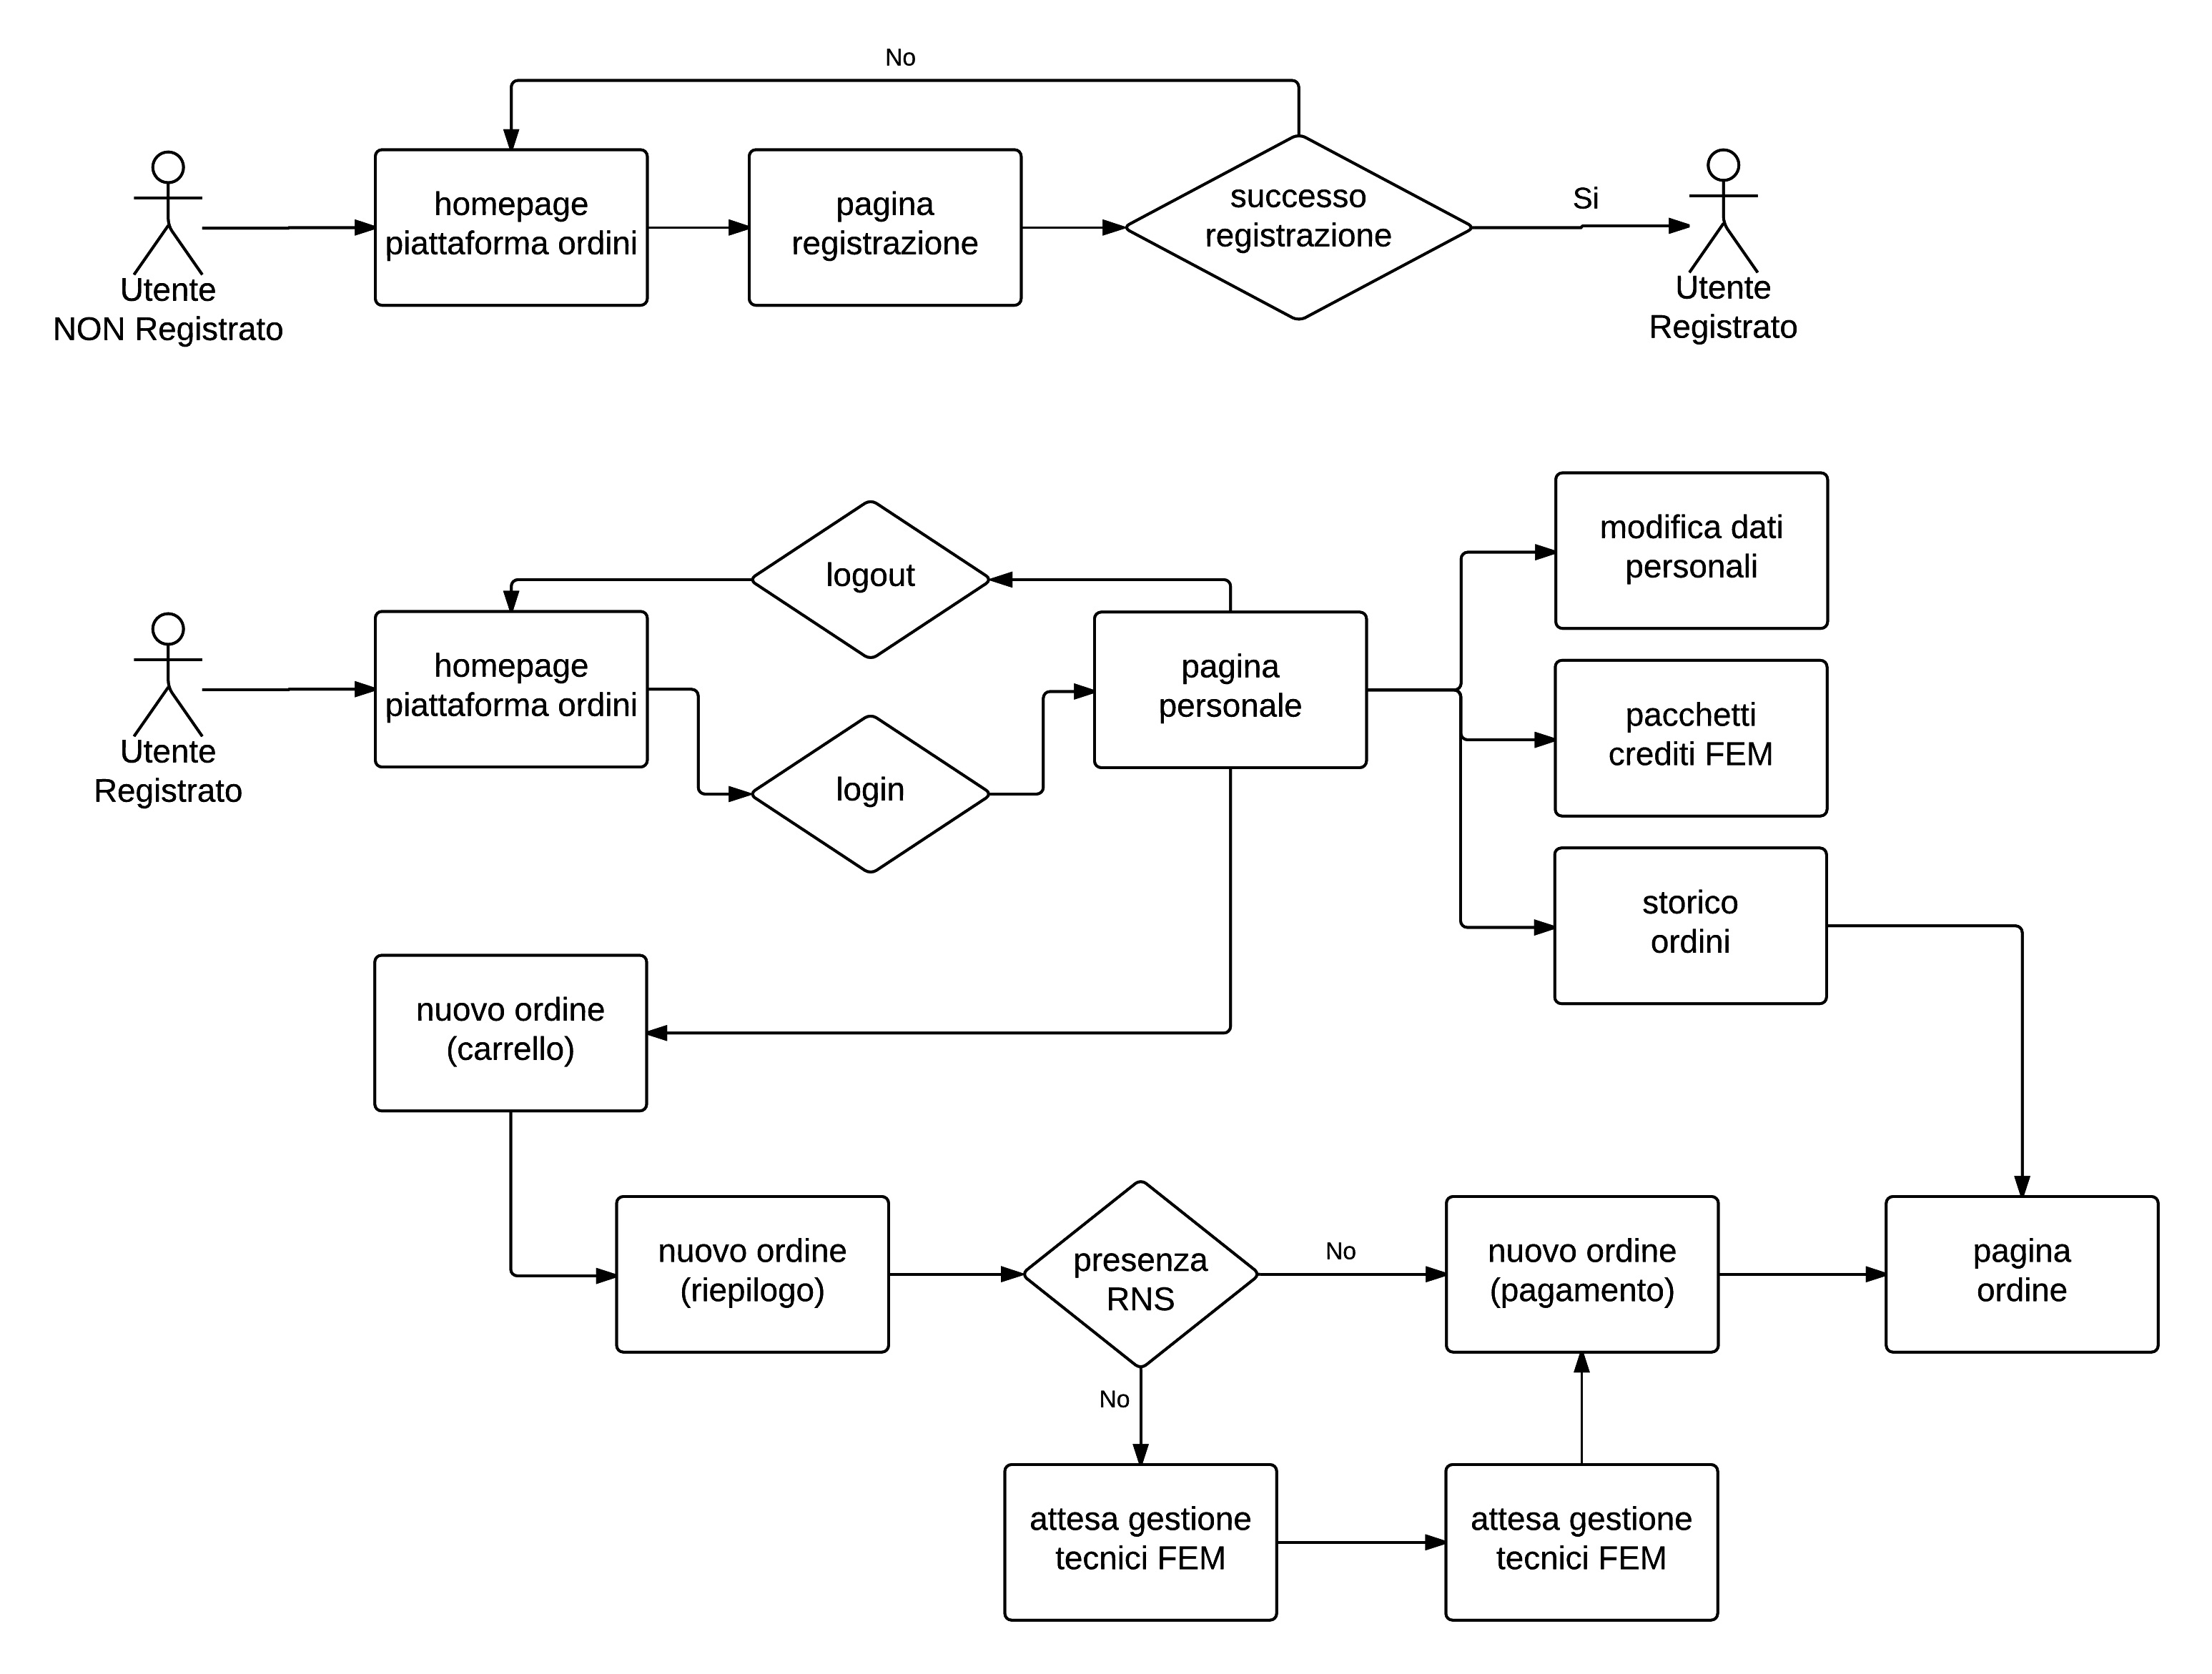
\includegraphics[width=1\textwidth]{images/flusso-cliente} 
 \caption{flusso cliente}
 \label{fig:flusso-cliente}
\end{figure}

Sono stati quindi introdotti alcuni comandi:
\begin{itemize}
 \item per includere un file HTML all'interno di un altro
  \begin{verbatim} 
    
  \end{verbatim}
 \item per indicare un blocco di contenuto specifico; ad esempio inserendo \texttt{jsexec} al posto di '{\dots}' si indica una porzione dedicata a script {\js}, oppure scrivendo \texttt{title} si indica il titolo della pagina HTML
  \begin{verbatim} 
    
  \end{verbatim}
 \item per descrivere come il file HTML richieda di essere una estensione di un altro file (molto utile per creare e modificare lo stile di base di tutti i file generati in uno unico, in questo progetto chiamato \texttt{base.html}).
  \begin{verbatim} 
    
  \end{verbatim} 
\end{itemize}
Alcuni esempi di utilizzo sono mostrati nell'appendice~\ref{app:templates}.

Con la creazione del file \texttt{base.html} si sono definiti file statici come CSS e {\js} una sola volta, generando uno stile solido e centralizzato che permette però personalizzazioni.

Dalla figura~\ref{fig:flusso-cliente} del flusso cliente si evince come il primo passo sia stato costruire una sorta di Homepage per introdurre i clienti non registrati al Portale (file chiamato \texttt{home.html}) e da qui, attraverso la barra di navigazione, dare la possibilità di effettuare il login o la registrazione.

\subsection*{registrazione e pagina personale}
\label{subs:preg-ppers}
La pagina di registrazione (\texttt{register.html}) ha richiesto l'utilizzo di codice {\js} principalmente per il controllo dei dati inseriti nei campi del form; in particolare il controllo in browser della compilazione di tutti i campi obbligatori e della loro correttezza sintattica in modo da evitare inutili comunicazione con il server che porterebbero a una, seppur lieve, perdita di tempo.

I controlli sono dei semplici 'validatori' che assegnano \texttt{true} alla variabile \texttt{any\_error} in modo da visualizzare un messaggio di errore al momento dell'invio del form. Per rendere ancora più esplicito il messaggio di errore é stato inserito in un \emph{modale}, strumento introdotto da {\b} che consiste in un \tag{div} al centro della viewport (ovvero la regione di pagina che viene visualizzata nel monitor) che monopolizza l'attenzione. All'interno di esso viene inserito il testo relativo all'errore. Ad esempio
\begin{verbatim}
if(any_error) {
 modal
  .body("Sono presenti alcuni errori")
}
\end{verbatim}

Una volta completato il processo di registrazione il cliente visualizza la propria pagina personale (figura~\ref{fig:ppersonale}) in cui può vedere la propria cronologia di ordini, modificare i dati personali, acquistare pacchetti crediti FEM, ma soprattutto creare un nuovo ordine.

\begin{figure}
 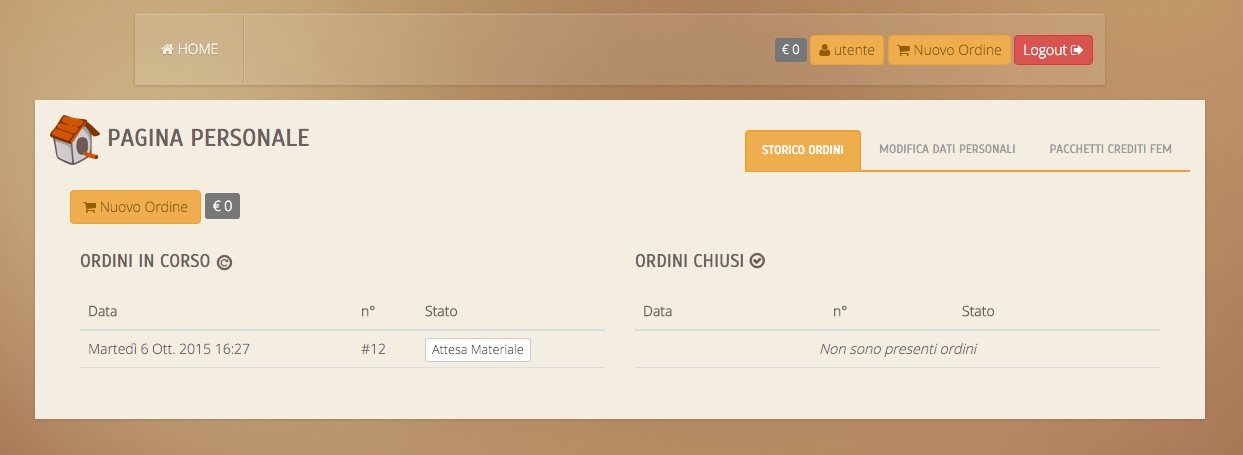
\includegraphics[width=1\textwidth]{images/ppersonale} 
 \caption{pagina personale}
 \label{fig:ppersonale}
\end{figure}

\subsection*{nuovo ordine}
\label{subs:pno}
La pagina di creazione dell'ordine é divisa in tre blocchi come sono le sue fasi: \emph{carrello}, \emph{riepilogo}, \emph{pagamento}.

La prima schermata del carrello é divisa in due parti (figura˜\ref{fig:pno-cart}). In alto si trova la tabella che funge da carrello vero e proprio raccogliendo tutti i campioni inseriti dal cliente e mostrando i relativi dati associati come identificativo, specie, analisi richieste, costo, etc. In basso si trova il form per l'inserimento di dei soggetti.

\begin{figure}
 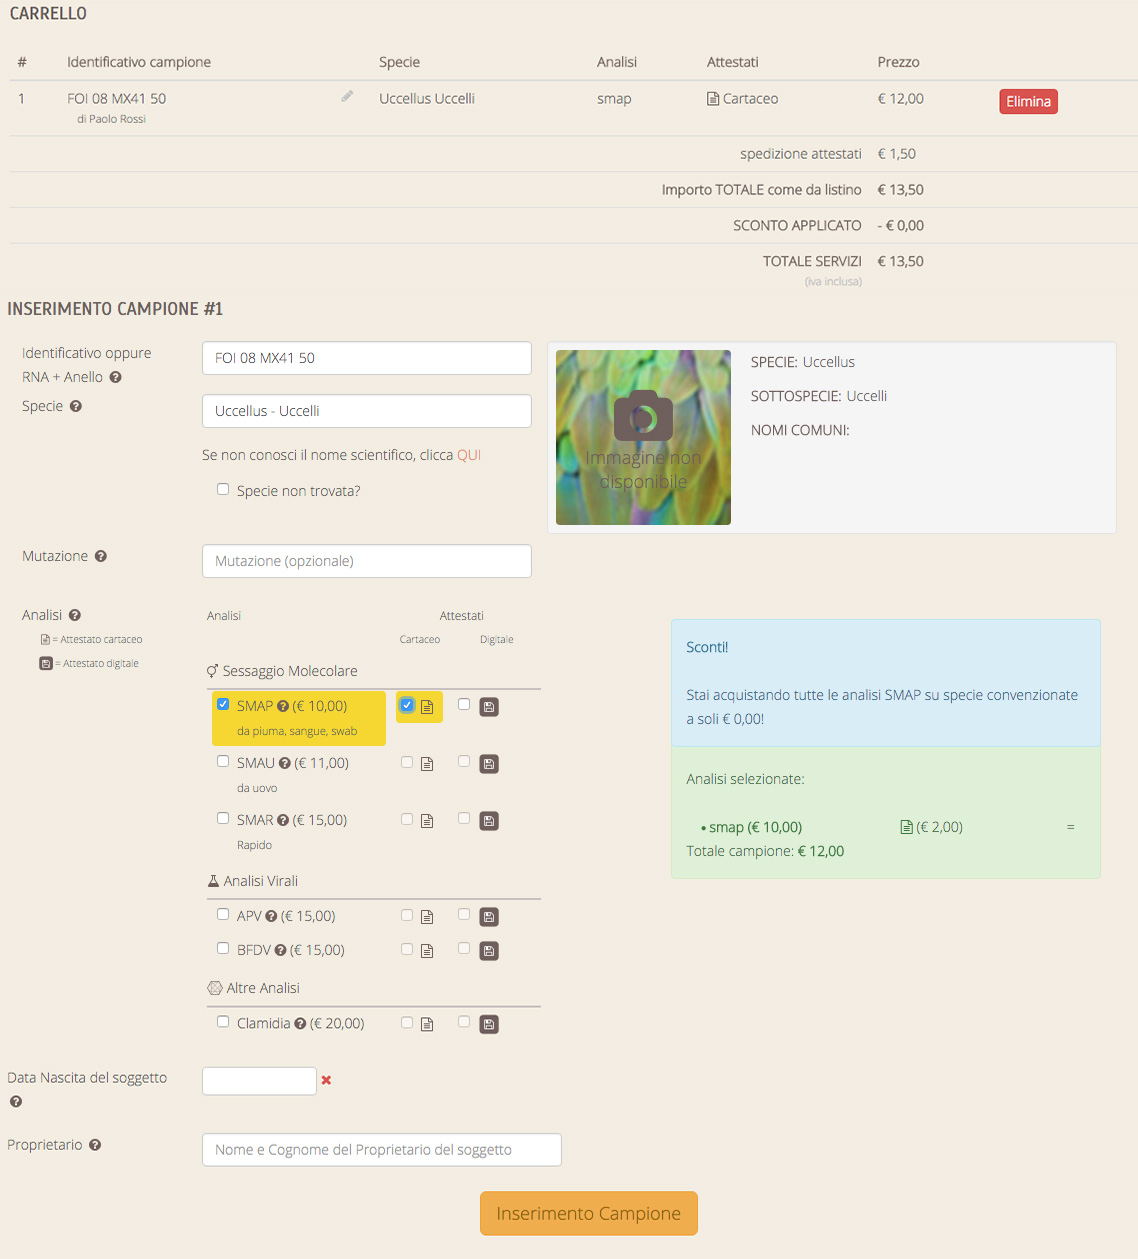
\includegraphics[width=1\textwidth]{images/pno-cart} 
 \caption{nuovo ordine - schermata carrello}
 \label{fig:pno-cart}
\end{figure}

Come nella pagina di registrazione viene utilizzato del codice {\js} per la validazione dei campi, inoltre il campo \texttt{specie} funge da elenco in cui cercare la specie/sottospecie del soggetto. 

Una volta selezionata la specie, a destra verrà popolato un \tag{div} (identificato dalla classe \texttt{taxonomy})contenente l'immagine e altre informazioni come i nome comuni come descritto nel seguente estratto di codice; se non é stata correttamente selezionata la specie tra quelle esistenti  il \tag{div} \texttt{taxonomy} non deve comparire. Per farlo é stata creata una classe apposta in CSS (\texttt{dno}) che va a impostare \texttt{display:none}, cioè oggetto non visibile. Di seguito se la specie é stata selezionata correttamente si popolano gli appositi \tag{div} innestati (identificati dagli \texttt{id="nome\_specie"} e così via) e l'immagine; quest'ultima potrebbe non essere presente per alcune specie, in questi casi si caricherà un immagine preimpostata per indicarlo.

\begin{footnotesize}
\begin{verbatim}
  if($(this).val() == "-1") {
    $(".taxonomy").addClass("dno");
  } else {
    if(data_Specie[$(this).val()].immagine == "") {
      $(".image-exist").addClass("dno");
      $(".image-not-exist").removeClass("dno");
    } else {
      $(".image-exist").attr
       ("src" "/media/"+data_Specie[$(this).val()].immagine).removeClass("dno");
      $(".image-not-exist").addClass("dno");
    }
    $("#nome_specie").html(data_Specie[$(this).val()].specie_padre)
    $("#nome_sottospecie").html(data_Specie[$(this).val()].nome);
    $("#nome_comune_sottospecie").html(data_Specie[$(this).val()].nome_comune);
    $(".taxonomy").removeClass("dno");
  } 
 
\end{verbatim}
\end{footnotesize}

Una volta completata l'aggiunta di soggetti si passa al \emph{riepilogo}, sezione nella quale viene riproposto l'elenco completo degli esemplari aggiunti da analizzare, e richiesta l'eventuale aggiunta di campioni standard in caso di specie classificate come junior.

Infine si visualizza la schermata per il pagamento nella quale si sceglie attraverso \texttt{checkbox} la modalità preferita e dinamicamente vengono descritte in un \tag{div} le coordinate per i pagamenti e per la spedizione delle piume.

Durante la creazione di un ordine può esserci un passo in più, ovvero nel caso di selezione di una specie non presente nell'elenco fornito da {\fem} l'ordine viene arrestato, in attesa che un addetto dell'azienda classifichi correttamente la 'nuova specie' indicata dal cliente. Questo avviene sia per una questione di ordine e controllo, sia per mantenere la totale correttezza al momento della generazione degli attestati ed evitare di generare documentazione con specie non esistente e scritta in modo scorretto a causa di una svista.

\subsection*{ordine}
\label{subs:po}
Completato l'ordine il cliente viene indirizzato al pagina dedicata, in cui vengono riproposte le coordinate di pagamento se non é ancora stato eseguito l'elenco dei soggetti da analizzare, lo stato delle analisi, la possibilità di scaricare gli attestati digitali e una sezione dedicata alla comunicazione diretta con {\fem} (figura~\ref{fig:po}).

\begin{figure}
 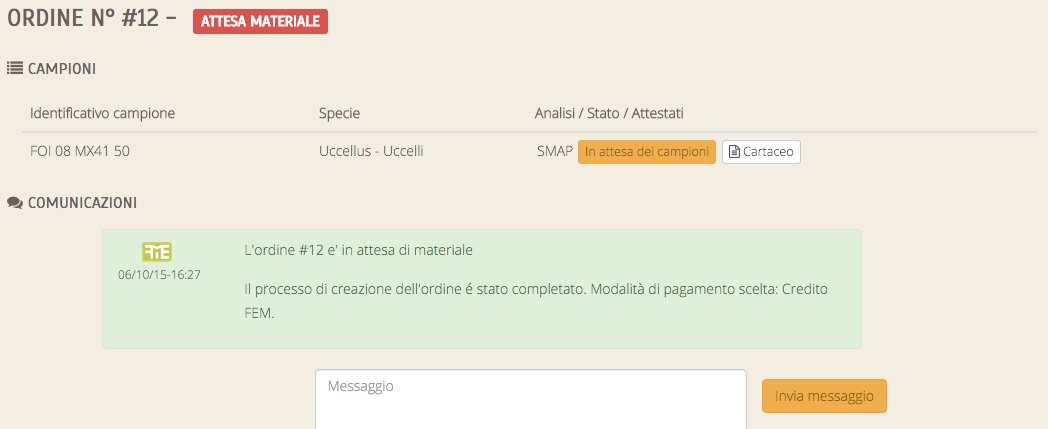
\includegraphics[width=1\textwidth]{images/po} 
 \caption{pagina ordine}
 \label{fig:po}
\end{figure}

\newpage
\subsection{Vista Admin}
\label{subs:admin}

\begin{wrapfigure}{l}{0.27\textwidth}
  \begin{center}
    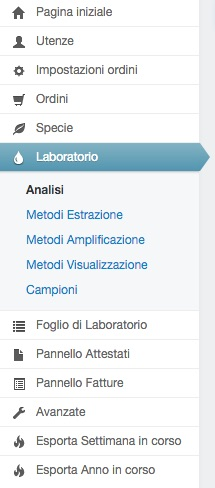
\includegraphics[width=0.25\textwidth]{images/suit}
  \end{center}
\end{wrapfigure}

Il controllo del flusso ordini e la comunicazione con il cliente sono una facciata importantissima per un e-commerce, e per questo motivo é necessaria una efficace interfaccia utente per l'utilizzo della piattaforma in tutte le sue potenzialità.

Django mette a disposizione un pannello admin autogenerato basato sui modelli definiti (vedi~\ref{subs:crea}), ma per una migliore usabilità abbiamo deciso di installare \emph{Django Suit}, una estensione per un tema alternativo del pannello admin dei sistemi Django \cite{suit}. Django Suit ci ha permesso di personalizzare il lato admin andando incontro alle richieste dei tecnici di {\fem}. A lato si può vedere la barra verticale di navigazione.

Gli utenti lato admin, cioè dipendenti di {\fem}, si possono dividere in due tipologie: gli addetti al controllo e ai rapporti con la clientela, e i tecnici di laboratorio.

I primi controlleranno le utenze, i dati della clientela, i prezzi e la scontistica legata o non legata alle associazioni convenzionate, le statistiche e la messaggistica con il cliente.

I secondi si occuperanno di effettuare le analisi, controllare il corretto flusso degli ordini e la generazione degli attestati.

Il dettaglio delle azioni lato admin sono descritte nell'appendice~\ref{app:admin}.

La configurazione di Django Suit avviene come segue
\begin{footnotesize}
\begin{verbatim}
 SUIT_CONFIG = {
    'ADMIN_NAME': 'Pannello admin del Portale Avifauna',
    'MENU': (
        'sites',
        {'label': 'Laboratorio', 'icon':'icon-tint', 
              'models': (
                   'ordini.analisi', 
                   'ordini.metodoestrazione', 
                   'ordini.metodoamplificazione', 
                   ordini.metodovisualizzazione', 
                   'ordini.campione')},
    ),
 }
\end{verbatim}
\end{footnotesize}

